\documentclass[12pt,addpoints,answers]{exam}
\usepackage[margin=1in]{geometry}
\usepackage{amsmath,amssymb,amsfonts}
\usepackage{graphicx}
\usepackage{float}
\usepackage[T1]{fontenc}
\usepackage[utf8]{inputenc}
\printanswers
\unframedsolutions

\begin{document}
\begin{center}
{\Large AP FRQ Pack}
\end{center}
\begin{questions}
\question
% q01-sgp02
People enter a line for an escalator at a rate modeled by the function $r$ given by \par $$r(t) = \begin{cases} 44\left(\frac{t}{100}\right)^3\left(1 - \frac{t}{300}\right)^7 & \text{for } 0 \le t \le 300 \\ 0 & \text{for } t > 300 \end{cases}$$ \par where $r(t)$ is measured in people per second and $t$ is measured in seconds. As people get on the escalator, they exit the line at a constant rate of 0.7 person per second. There are 20 people in line at time $t = 0$.
\begin{parts}
\part How many people enter the line for the escalator during the time interval $0 \le t \le 300$?
\part During the time interval $0 \le t \le 300$, there are always people in line for the escalator. How many people are in line at time $t = 300$?
\part For $t > 300$, what is the first time $t$ that there are no people in line for the escalator?
\part For $0 \le t \le 300$, at what time $t$ is the number of people in line a minimum? To the nearest whole number, find the number of people in line at this time. Justify your answer.
\end{parts}
\begin{solution}
Part (a): $\int_0^{300} r(t)\,dt = 270$ \par According to the model, 270 people enter the line for the escalator during the time interval $0 \le t \le 300$. \par Part (b): $20 + \int_0^{300} (r(t) - 0.7)\,dt = 20 + \int_0^{300} r(t)\,dt - 0.7 \cdot 300 = 80$ \par According to the model, 80 people are in line at time $t = 300$. \par Part (c): Based on part (b), the number of people in line at time $t = 300$ is 80. \par The first time $t$ that there are no people in line is $300 + \frac{80}{0.7} = 414.286$ (or 414.285) seconds. \par Part (d): The total number of people in line at time $t$, $0 \le t \le 300$, is modeled by $20 + \int_0^t r(x)\,dx - 0.7t$. \par $r(t) - 0.7 = 0 \Rightarrow t_1 = 33.013298, t_2 = 166.574719$ \par \[\begin{array}{c|c} t & \text{People in line for escalator} \\ \hline 0 & 20 \\ t_1 & 3.803 \\ t_2 & 158.070 \\ 300 & 80 \end{array}\] \par The number of people in line is a minimum at time $t = 33.013$ seconds, when there are 4 people in line.
\begin{center}
\begin{tabular}{|l|l|}
\hline
$t$ & People in line for escalator \\
\hline
0 & 20 \\
\hline
$t_1$ & 3.803 \\
\hline
$t_2$ & 158.070 \\
\hline
300 & 80 \\
\hline
\end{tabular}
\end{center}
\par\medskip
\textbf{Scoring Guide}\par
Part (a): 2 points: $\{1 : integral, 1 : answer\}$ Part (b): 2 points: $\{1 : considers rate out, 1 : answer\}$ Part (c): 1 point: $\{1 : answer\}$ Part (d): 4 points: $\{1 : considers r(t) - 0.7 = 0, 1 : identifies t = 33.013, 1 : answers, 1 : justification\}$
\end{solution}

\question
% q02-sgp03
Researchers on a boat are investigating plankton cells in a sea. At a depth of $h$ meters, the density of plankton cells, in millions of cells per cubic meter, is modeled by $p(h) = 0.2h^2 e^{-0.0025h^2}$ for $0 \le h \le 30$ and is modeled by $f(h)$ for $h \ge 30$. The continuous function $f$ is not explicitly given.
\begin{parts}
\part Find $p'(25)$. Using correct units, interpret the meaning of $p'(25)$ in the context of the problem.
\part Consider a vertical column of water in this sea with horizontal cross sections of constant area 3 square meters. To the nearest million, how many plankton cells are in this column of water between $h = 0$ and $h = 30$ meters?
\part There is a function $u$ such that $0 \le f(h) \le u(h)$ for all $h \ge 30$ and $\int_{30}^{\infty} u(h)\,dh = 105$. The column of water in part (b) is $K$ meters deep, where $K > 30$. Write an expression involving one or more integrals that gives the number of plankton cells, in millions, in the entire column. Explain why the number of plankton cells in the column is less than or equal to 2000 million.
\part The boat is moving on the surface of the sea. At time $t \ge 0$, the position of the boat is $(x(t), y(t))$, where $x'(t) = 662\sin(5t)$ and $y'(t) = 880\cos(6t)$. Time $t$ is measured in hours, and $x(t)$ and $y(t)$ are measured in meters. Find the total distance travelled by the boat over the time interval $0 \le t \le 1$.
\end{parts}
\begin{solution}
Part (a): $p'(25) = -1.179$ \par At a depth of 25 meters, the density of plankton cells is changing at a rate of $-1.179$ million cells per cubic meter per meter. \par Part (b): $\int_0^{30} 3p(h)\,dh = 1675.414936$ \par There are 1675 million plankton cells in the column of water between $h = 0$ and $h = 30$ meters. \par Part (c): $\int_{30}^K 3f(h)\,dh$ represents the number of plankton cells, in millions, in the column of water from a depth of 30 meters to a depth of $K$ meters. \par The number of plankton cells, in millions, in the entire column of water is given by $\int_0^{30} 3p(h)\,dh + \int_{30}^K 3f(h)\,dh$. \par Because $0 \le f(h) \le u(h)$ for all $h \ge 30$, $$3\int_{30}^K f(h)\,dh \le 3\int_{30}^K u(h)\,dh \le 3\int_{30}^\infty u(h)\,dh = 3 \cdot 105 = 315.$$ \par The total number of plankton cells in the column of water is bounded by $1675.415 + 315 = 1990.415 \le 2000$ million. \par Part (d): $\int_0^1 \sqrt{(x'(t))^2 + (y'(t))^2}\,dt = 757.455862$ \par The total distance traveled by the boat over the time interval $0 \le t \le 1$ is 757.456 (or 757.455) meters.
\par\medskip
\textbf{Scoring Guide}\par
Part (a): 2 points: 1 point for answer; 1 point for meaning with units. Part (b): 2 points: 1 point for integrand; 1 point for answer. Part (c): 3 points: 1 point for integral expression; 1 point for compares improper integral; 1 point for explanation. Part (d): 2 points: 1 point for integrand; 1 point for total distance.
\end{solution}

\question
% q03-sgp04
The graph of the continuous function $g$, the derivative of the function $f$, is shown above. The function $g$ is piecewise linear for $-5 \le x < 3$, and $g(x) = 2(x - 4)^2$ for $3 \le x \le 6$.
\begin{center}
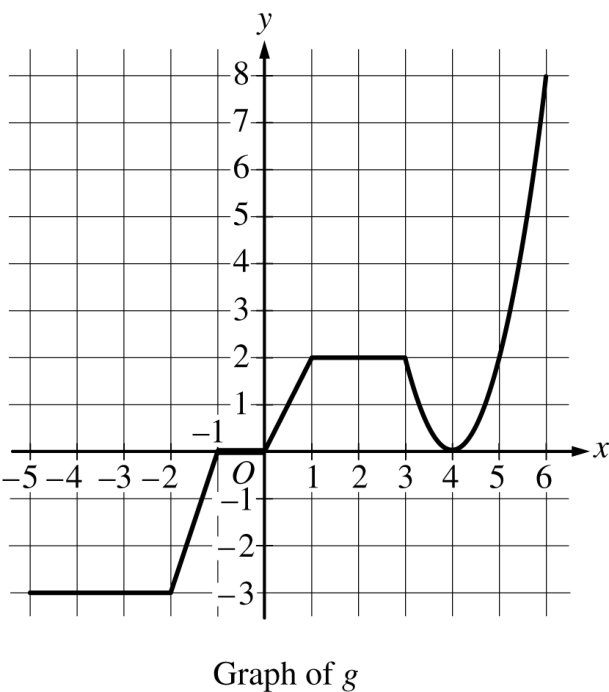
\includegraphics[width=0.8\linewidth]{figures/BC-2018_q3_fig_1.png}
\\ Graph of $g$
\end{center}
\begin{parts}
\part If $f(1) = 3$, what is the value of $f(-5)$?
\part Evaluate $\int_1^6 g(x)\,dx$.
\part For $-5 < x < 6$, on what open intervals, if any, is the graph of $f$ both increasing and concave up? Give a reason for your answer.
\part Find the $x$-coordinate of each point of inflection of the graph of $f$. Give a reason for your answer.
\end{parts}
\begin{solution}
Part (a): $f(-5) = f(1) + \int_{1}^{-5} g(x)\,dx = f(1) - \int_{-5}^{1} g(x)\,dx = 3 - \left(-9 - \frac{3}{2} + 1\right) = 3 - \left(-\frac{19}{2}\right) = \frac{25}{2}$ \par Part (b): $\int_{1}^{6} g(x)\,dx = \int_{1}^{3} g(x)\,dx + \int_{3}^{6} g(x)\,dx = \int_{1}^{3} 2\,dx + \int_{3}^{6} 2(x-4)^2\,dx = 4 + \left[\frac{2}{3}(x-4)^3\right]_{x=3}^{x=6} = 4 + \frac{16}{3} - \left(-\frac{2}{3}\right) = 10$ \par Part (c): The graph of $f$ is increasing and concave up on $0 < x < 1$ and $4 < x < 6$ because $f'(x) = g(x) > 0$ and $f''(x) = g'(x)$ is increasing on those intervals. \par Part (d): The graph of $f$ has a point of inflection at $x = 4$ because $f''(x) = g(x)$ changes from decreasing to increasing at $x = 4$.
\par\medskip
\textbf{Scoring Guide}\par
Part (a): 2 points: 1 point for integral setup/method, 1 point for answer of $\frac{25}{2}$ Part (b): 3 points: 1 point for split at $x = 3$; 1 point for antiderivative of $2(x-4)^2$; 1 point for answer of $10$ Part (c): 2 points: 1 point for identifying intervals $0 < x < 1$ and $4 < x < 6$; 1 point for valid reason (that $f'(x) = g(x) > 0$ and $f''(x) = g(x)$ is increasing) Part (d): 2 points: 1 point for answer $x = 4$; 1 point for reason that $f''(x) = g(x)$ changes from decreasing to increasing at $x = 4$
\end{solution}

\question
% q04-sgp05
The height of a tree at time $t$ is given by a twice-differentiable function $H$, where $H(t)$ is measured in meters and $t$ is measured in years. Selected values of $H(t)$ are given in the table above.
\begin{center}
\begin{tabular}{|l|l|l|l|l|l|}
\hline
$t$ (years) & 2 & 3 & 5 & 7 & 10 \\
\hline
$H(t)$ (meters) & 1.5 & 2 & 6 & 11 & 15 \\
\hline
\end{tabular}
\end{center}
\begin{parts}
\part Use the data in the table to estimate $H'(6)$. Using correct units, interpret the meaning of $H'(6)$ in the context of the problem.
\part Explain why there must be at least one time $t$, for $2 < t < 10$, such that $H'(t) = 2$.
\part Use a trapezoidal sum with the four subintervals indicated by the data in the table to approximate the average height of the tree over the time interval $2 \le t \le 10$.
\part The height of the tree, in meters, can also be modeled by the function $G$, given by $G(x) = \frac{100x}{1 + x}$, where $x$ is the diameter of the base of the tree, in meters. When the tree is 50 meters tall, the diameter of the base of the tree is increasing at a rate of 0.03 meter per year. According to this model, what is the rate of change of the height of the tree with respect to time, in meters per year, at the time when the tree is 50 meters tall?
\end{parts}
\begin{solution}
Part (a): $H'(6) \approx \frac{H(7) - H(5)}{7-5} = \frac{11-6}{2} = \frac{5}{2}$ \par $H'(6)$ is the rate at which the height of the tree is changing, in meters per year, at time $t = 6$ years. \par Part (b): $\frac{H(5) - H(3)}{5-3} = \frac{6-2}{2} = 2$ \par Because $H$ is differentiable on $3 \le t \le 5$, $H$ is continuous on $3 \le t \le 5$. \par By the Mean Value Theorem, there exists a value $c$, $3 < c < 5$, such that $H'(c) = 2$. \par Part (c): The average height of the tree over the time interval $2 \le t \le 10$ is given by \par $$\frac{1}{10-2}\int_2^{10} H(t)\,dt$$ \par $$\frac{1}{8}\int_2^{10} H(t)\,dt \approx \frac{1}{8}\left(\frac{1.5+2}{2}\cdot 1 + \frac{2+6}{2}\cdot 2 + \frac{6+11}{2}\cdot 2 + \frac{11+15}{2}\cdot 2 + 3\right)$$ \par $$= \frac{1}{8}(65.75) = \frac{263}{32}$$ \par The average height of the tree over the time interval $2 \le t \le 10$ is $\frac{263}{32}$ meters. \par Part (d): $G(x) = 50 \Rightarrow x = 1$ \par $$\frac{d}{dt}(G(x)) = \frac{d}{dx}(G(x)) \cdot \frac{dx}{dt} = \frac{(1+x) \cdot 100 - 100x \cdot 1}{(1+x)^2} \cdot \frac{dx}{dt} = \frac{100}{(1+x)^2} \cdot \frac{dx}{dt}$$ \par $$\frac{d}{dt}(G(x))\bigg|_{x=1} = \frac{100}{(1+1)^2} \cdot 0.03 = \frac{3}{4}$$ \par According to the model, the rate of change of the height of the tree with respect to time when the tree is 50 meters tall is $\frac{3}{4}$ meter per year.
\par\medskip
\textbf{Scoring Guide}\par
Part (a): 2 points 1 point: estimate 1 point: interpretation with units Part (b): 2 points 1 point: $\frac{H(5) - H(3)}{5-3}$ 1 point: conclusion using Mean Value Theorem Part (c): 2 points 1 point: trapezoidal sum 1 point: approximation Part (d): 3 points 2 points: $\frac{d}{dt}(G(x))$ 1 point: answer Note: max 1/3 [1-0] if no chain rule
\end{solution}

\question
% q05-sgp06
The graphs of the polar curves $r = 4$ and $r = 3 + 2\cos\theta$ are shown in the figure above. The curves intersect at $\theta = \frac{\pi}{3}$ and $\theta = \frac{5\pi}{3}$.
\begin{center}
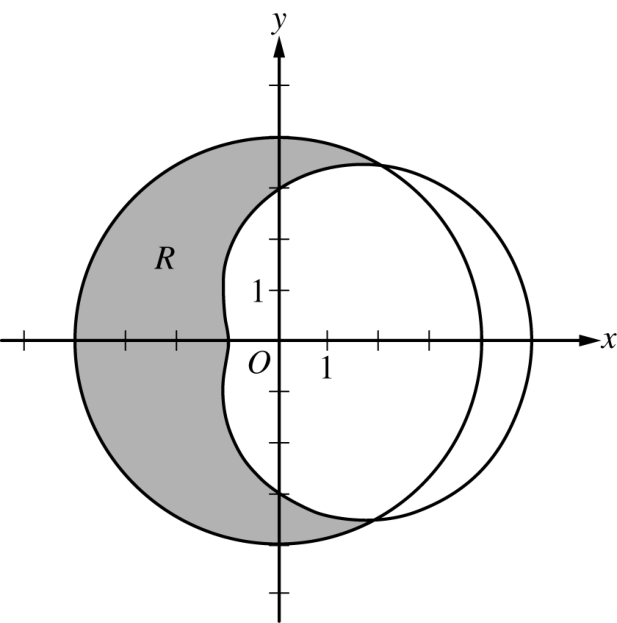
\includegraphics[width=0.8\linewidth]{figures/BC-2018_q5_fig_1.png}
\end{center}
\begin{parts}
\part Let $R$ be the shaded region that is inside the graph of $r = 4$ and also outside the graph of $r = 3 + 2\cos\theta$, as shown in the figure above. Write an expression involving an integral for the area of $R$.
\part Find the slope of the line tangent to the graph of $r = 3 + 2\cos\theta$ at $\theta = \frac{\pi}{2}$.
\part A particle moves along the portion of the curve $r = 3 + 2\cos\theta$ for $0 < \theta < \frac{\pi}{2}$. The particle moves in such a way that the distance between the particle and the origin increases at a constant rate of 3 units per second. Find the rate at which the angle $\theta$ changes with respect to time at the instant when the position of the particle corresponds to $\theta = \frac{\pi}{3}$. Indicate units of measure.
\end{parts}
\begin{solution}
Part (a): Area $= \frac{1}{2}\int_{\pi/3}^{5\pi/3} \left(4^2 - (3 + 2\cos\theta)^2\right) d\theta$ \par Part (b): $\frac{dr}{d\theta} = -2\sin\theta \Rightarrow \left.\frac{dr}{d\theta}\right|_{\theta=\pi/2} = -2$ \par $r\left(\frac{\pi}{2}\right) = 3 + 2\cos\left(\frac{\pi}{2}\right) = 3$ \par $y = r\sin\theta \Rightarrow \frac{dy}{d\theta} = \frac{dr}{d\theta}\sin\theta + r\cos\theta$ \par $x = r\cos\theta \Rightarrow \frac{dx}{d\theta} = \frac{dr}{d\theta}\cos\theta - r\sin\theta$ \par $\left.\frac{dy}{dx}\right|_{\theta=\pi/2} = \frac{dy/d\theta\big|_{\theta=\pi/2}}{dx/d\theta\big|_{\theta=\pi/2}} = \frac{-2\sin\left(\frac{\pi}{2}\right) + 3\cos\left(\frac{\pi}{2}\right)}{-2\cos\left(\frac{\pi}{2}\right) - 3\sin\left(\frac{\pi}{2}\right)} = \frac{2}{3}$ \par The slope of the line tangent to the graph of $r = 3 + 2\cos\theta$ at $\theta = \frac{\pi}{2}$ is $\frac{2}{3}$. \par — OR — \par $y = r\sin\theta = (3 + 2\cos\theta)\sin\theta \Rightarrow \frac{dy}{d\theta} = 3\cos\theta + 2\cos^2\theta - 2\sin^2\theta$ \par $x = r\cos\theta = (3 + 2\cos\theta)\cos\theta \Rightarrow \frac{dx}{d\theta} = -3\sin\theta - 4\sin\theta\cos\theta$ \par $\left.\frac{dy}{dx}\right|_{\theta=\pi/2} = \frac{dy/d\theta\big|_{\theta=\pi/2}}{dx/d\theta\big|_{\theta=\pi/2}} = \frac{3\cos\left(\frac{\pi}{2}\right) + 2\cos^2\left(\frac{\pi}{2}\right) - 2\sin^2\left(\frac{\pi}{2}\right)}{-3\sin\left(\frac{\pi}{2}\right) - 4\sin\left(\frac{\pi}{2}\right)\cos\left(\frac{\pi}{2}\right)} = \frac{2}{3}$ \par The slope of the line tangent to the graph of $r = 3 + 2\cos\theta$ at $\theta = \frac{\pi}{2}$ is $\frac{2}{3}$. \par Part (c): $\frac{dr}{dt} = \frac{dr}{d\theta}\frac{d\theta}{dt} = -2\sin\theta \cdot \frac{d\theta}{dt} \Rightarrow \frac{d\theta}{dt} = \frac{dr/dt}{-2\sin\theta}$ \par $\left.\frac{d\theta}{dt}\right|_{\theta=\pi/3} = 3 \cdot \frac{1}{-2\sin\left(\frac{\pi}{3}\right)} = \frac{3}{-\sqrt{3}} = -\sqrt{3}$ radians per second
\par\medskip
\textbf{Scoring Guide}\par
Part (a): 3 points: - 1 point: constant and limits - 2 points: integrand Part (b): 3 points: - 1 point: $\frac{dy}{d\theta} = \frac{dr}{d\theta}\sin\theta + r\cos\theta$ or $\frac{dx}{d\theta} = \frac{dr}{d\theta}\cos\theta - r\sin\theta$ - 1 point: $\frac{dy}{d\theta} = \frac{dr}{d\theta}\sin\theta + r\cos\theta$ or $\frac{dx}{d\theta} = \frac{dr}{d\theta}\cos\theta - r\sin\theta$ - 1 point: answer Part (c): 3 points: - 1 point: $\frac{dr}{dt} = \frac{dr}{d\theta}\frac{d\theta}{dt}$ - 1 point: $\frac{d\theta}{dt} = \frac{dr/dt}{-2\sin\theta}$ - 1 point: answer with units
\end{solution}

\question
% q06-sgp07
The Maclaurin series for $\ln(1 + x)$ is given by $$x - \frac{x^2}{2} + \frac{x^3}{3} - \frac{x^4}{4} + \cdots + (-1)^{n+1}\frac{x^n}{n} + \cdots$$ \par On its interval of convergence, this series converges to $\ln(1 + x)$. Let $f$ be the function defined by $$f(x) = x \ln\left(1 + \frac{x}{3}\right).$$
\begin{parts}
\part Write the first four nonzero terms and the general term of the Maclaurin series for $f$.
\part Determine the interval of convergence of the Maclaurin series for $f$. Show the work that leads to your answer.
\part Let $P_4(x)$ be the fourth-degree Taylor polynomial for $f$ about $x = 0$. Use the alternating series error bound to find an upper bound for $\left|P_4(2) - f(2)\right|$.
\end{parts}
\begin{solution}
Part (a): The first four nonzero terms are $\frac{x^2}{3} - \frac{x^3}{2 \cdot 3^2} + \frac{x^4}{3 \cdot 3^3} - \frac{x^5}{4 \cdot 3^4}$. \par The general term is $(-1)^{n+1} \frac{x^{n+1}}{n \cdot 3^n}$. \par Part (b): $$\lim_{n \to \infty} \left| \frac{(-1)^{n+2} x^{n+2}}{(n+1)(3^{n+1})} \cdot \frac{n \cdot 3^n}{(-1)^{n+1} x^{n+1}} \right| = \lim_{n \to \infty} \left| \frac{-x}{3} \cdot \frac{n}{(n+1)} \right| = \left| \frac{x}{3} \right|$$ \par $\left| \frac{x}{3} \right| < 1$ for $|x| < 3$ \par Therefore, the radius of convergence of the Maclaurin series for $f$ is $3$. \par — OR — \par The radius of convergence of the Maclaurin series for $\ln(1 + x)$ is $1$, so the series for $f(x) = x \ln\left(1 + \frac{x}{3}\right)$ converges absolutely for $\left| \frac{x}{3} \right| < 1$. \par $\left| \frac{x}{3} \right| < 1 \Rightarrow |x| < 3$ \par Therefore, the radius of convergence of the Maclaurin series for $f$ is $3$. \par When $x = -3$, the series is $\sum_{n=1}^{\infty} (-1)^{n+1} \frac{(-3)^{n+1}}{n \cdot 3^n} = \sum_{n=1}^{\infty} \frac{3}{n}$, which diverges by comparison to the harmonic series. \par When $x = 3$, the series is $\sum_{n=1}^{\infty} (-1)^{n+1} \frac{3^{n+1}}{n \cdot 3^n} = \sum_{n=1}^{\infty} (-1)^{n+1} \frac{3}{n}$, which converges by the alternating series test. \par The interval of convergence of the Maclaurin series for $f$ is $-3 < x \le 3$. \par Part (c): By the alternating series error bound, an upper bound for $|P_4(2) - f(2)|$ is the magnitude of the next term of the alternating series. \par $$|P_4(2) - f(2)| < \left| -\frac{2^5}{4 \cdot 3^4} \right| = \frac{8}{81}$$
\par\medskip
\textbf{Scoring Guide}\par
Part (a): 2 points 1 : first four terms 1 : general term Part (b): 5 points 1 : sets up ratio 1 : computes limit of ratio 1 : radius of convergence 1 : considers both endpoints 1 : analysis and interval of convergence — OR — 1 : radius for $\ln(1+x)$ series 1 : substitutes $\frac{x}{3}$ 1 : radius of convergence 1 : considers both endpoints 1 : analysis and interval of convergence Part (c): 2 points 1 : uses fifth-degree term as error bound 1 : answer
\end{solution}
\end{questions}
\end{document}
